\documentclass[12pt, a4paper]{report}
\renewcommand{\baselinestretch}{2.0}

\usepackage[T1]{fontenc}
\usepackage{times,newtxmath,newtxtext}
\usepackage[utf8]{inputenc}
\usepackage{subcaption}
\usepackage{setspace}
\usepackage{multirow}
\usepackage{multicol}
\usepackage[tableposition=top]{caption}
\usepackage[table,xcdraw]{xcolor}
\usepackage{titlesec}
\usepackage{indentfirst}
\usepackage{enumitem}
\usepackage{overpic}
\usepackage{tikz}

\setlength{\parindent}{1cm}

\captionsetup[table]{labelsep=space}
\captionsetup[figure]{labelsep=space}

\usetikzlibrary{shapes.geometric, arrows}
\definecolor{blu}{RGB}{135,206,250}
\definecolor{ore}{RGB}{255,140,0}
\tikzstyle{process} = [rectangle, rounded corners, minimum width=4cm, minimum height=1cm, text centered, text width=5cm, draw=black, fill=blu]
\tikzstyle{process2} = [rectangle, rounded corners, minimum width=3cm, minimum height=1cm, text centered, text width=3cm, draw=black, fill=blu]
\tikzstyle{decision} = [diamond, minimum width=2.2cm, minimum height=0.3cm, text centered, text width=1.1cm, draw=black, fill=orange!40]
\tikzstyle{arrow} = [thick,->,>=stealth]

\usepackage{gensymb}
\usepackage{notoccite}
\usepackage{float}
\usepackage{hyperref}
\hypersetup{
    colorlinks,
    citecolor=black,
    filecolor=black,
    linkcolor=black,
    urlcolor=black,
    linkbordercolor=red
}
\usepackage{indentfirst}
\usepackage{amsmath}
\renewcommand{\chaptername}{BAB }
\renewcommand{\figurename}{Gambar}
\renewcommand{\tablename}{Tabel}
\renewcommand{\contentsname}{DAFTAR ISI}
\renewcommand{\listtablename}{DAFTAR TABEL}
\renewcommand{\listfigurename}{DAFTAR GAMBAR}
\renewcommand{\bibname}{DAFTAR PUSTAKA}

\renewcommand{\thechapter}{\Roman{chapter}}
\renewcommand{\thesection}{\arabic{chapter}.\arabic{section}.}
\renewcommand{\thesubsection}{\arabic{chapter}.\arabic{section}.\arabic{subsection}.}
\renewcommand{\thesubsubsection}{\arabic{chapter}.\arabic{section}.\arabic{subsection}.\arabic{subsubsection}.}

\renewcommand{\thefigure}{\arabic{chapter}.\arabic{figure}}
\renewcommand{\thetable}{\arabic{chapter}.\arabic{table}}
\renewcommand{\theequation}{\arabic{chapter}.\arabic{equation}}

\usepackage{graphicx}
\usepackage[a4paper,top=40mm,bottom=30mm,left=40mm,right=30mm]{geometry}

\usepackage{tocloft}
\renewcommand{\cfttoctitlefont}{\hspace*{\fill}\Large\bfseries}
\renewcommand{\cftaftertoctitle}{\hspace*{\fill}}
\renewcommand{\cftlottitlefont}{\hspace*{\fill}\Large\bfseries}
\renewcommand{\cftafterlottitle}{\hspace*{\fill}}
\renewcommand{\cftloftitlefont}{\hspace*{\fill}\Large\bfseries}
\renewcommand{\cftafterloftitle}{\hspace*{\fill}}

\usepackage{sectsty}

\chapternumberfont{\Large} 
\chaptertitlefont{\Large}
\pagenumbering{roman}
\sectionfont{\normalsize}
\subsectionfont{\normalsize}
\titleformat{\section}{\large\bfseries}{\thesection}{1em}{}
\titlespacing\section{0pt}{12pt plus 4pt minus 2pt}{0pt plus 2pt minus 2pt}
\titlespacing\subsection{0pt}{12pt plus 4pt minus 2pt}{0pt plus 2pt minus 2pt}
\titlespacing\subsubsection{0pt}{12pt plus 4pt minus 2pt}{0pt plus 2pt minus 2pt}

\titleformat{\chapter}[display]
	{\normalfont\large\bfseries\centering}{\chaptertitlename \thechapter \centering}{-10pt}{\large}
\titlespacing*{\chapter}{0pt}{-30pt}{20pt}

\setcounter{secnumdepth}{4}
\setcounter{tocdepth}{4}

\usepackage{listings}
\usepackage{xcolor}
\definecolor{codegreen}{rgb}{0,0.6,0}
\definecolor{codegray}{rgb}{0.5,0.5,0.5}
\definecolor{codepurple}{rgb}{0.58,0,0.82}
\definecolor{backcolour}{rgb}{1,1,1}

\lstdefinestyle{mystyle}{
    backgroundcolor=\color{backcolour},   
    commentstyle=\color{codegreen},
    keywordstyle=\color{magenta},
    numberstyle=\tiny\color{codegray},
    stringstyle=\color{codepurple},
    basicstyle=\ttfamily\footnotesize,
    breakatwhitespace=false,         
    breaklines=true,                 
    captionpos=b,                    
    keepspaces=true,                 
    numbers=left,                    
    numbersep=5pt,                  
    showspaces=false,                
    showstringspaces=false,
    showtabs=false,                  
    tabsize=2
}

\lstset{style=mystyle}


\def\draftTitle{Efek Laser Merah dan Hijau Pada Hasil Pengukuran Partikel Berbasis Dynamic Light Scattering}
\def\fullName{Mohamad Fauzi}
\def\NPM{140310190053}
\def\dateOf{Desember 2023}
\def\laboratory{Instrumentasi}
\def\supervisorNameF{Ferry Faizal, Ph.D}
\def\NIPF{1234567 123456 1 123}
\def\supervisorNameS{Prof. Dr. Eng. I Made Joni, M.Sc}
\def\NIPS{1234567 123456 1 123}
\def\directorName{Prof. Dr. Eng. Camellia Panatarani, M.Si}
\def\NIPS{1234567 123456 1 123}

\title{major}
\author{\fullName}
\date{December 2023}

\begin{document}
    \newgeometry{a4paper,top=4cm,bottom=3cm,left=4cm,right=3cm}

    \begin{titlepage}
    \setstretch{1.5}
    \thispagestyle{empty}
    \begin{center}
        \begin{large}
            \begin{spacing}{1}
                \textbf{\MakeUppercase{\draftTitle}}
            \end{spacing}
        \end{large}

        \vspace{2cm}
        \textbf{SKRIPSI}

        \vspace{1cm}
        Diajukan sebagai Salah Satu Syarat untuk Menempuh Ujian Akhir Tingkat Sarjana pada Program Studi Fisika Fakultas Matematika dan Ilmu Pengetahuan Alam Universitas Padjadjaran
        
        \vspace{1cm}
        \textbf{\MakeUppercase{\fullName\\
        \NPM}}

        \vspace{2cm}
        \begin{figure}[h]
            \centering
            
\includegraphics[width=4cm]{Images/logo-unpad-fc.png}
            \label{fig:unpadlogo}
        \end{figure}

        \vspace{2cm}
        \textbf{PROGRAM STUDI FISIKA\\
        FAKULTAS MATEMATIKA DAN ILMU PENGETAHUAN ALAM\\
        UNIVERSITAS PADJADJARAN\\}

        \vspace{\baselineskip}
        \textbf{\large \the\year{}}
    \end{center}
\end{titlepage}
    \newpage
\begin{titlepage}
    \setstretch{1.5}
    \thispagestyle{empty}
    \begin{center}
        \begin{large}
            \begin{spacing}{1}
                \textbf{\MakeUppercase{\draftTitle}}
            \end{spacing}
        \end{large}

        \vspace{2cm}
        \textbf{SKRIPSI}

        \vspace{1cm}
        Diajukan sebagai Salah Satu Syarat untuk Menempuh Ujian Akhir Tingkat Sarjana pada Program Studi Fisika Fakultas Matematika dan Ilmu Pengetahuan Alam Universitas Padjadjaran
        
        \vspace{1cm}
        \textbf{\MakeUppercase{\fullName\\
        \NPM}}

        \vspace{2cm}
        \begin{figure}[h]
            \centering
            
\includegraphics[width=4cm]{Images/logo-unpad-bw.pdf}
            \label{fig:unpadlogo}
        \end{figure}

        \vspace{2cm}
        \textbf{PROGRAM STUDI FISIKA\\
        FAKULTAS MATEMATIKA DAN ILMU PENGETAHUAN ALAM\\
        UNIVERSITAS PADJADJARAN\\}

        \vspace{\baselineskip}
        \textbf{\large \the\year{}}
    \end{center}
\end{titlepage}
    \chapter*{\centering LEMBAR PENGESAHAN}
\addcontentsline{toc}{chapter}{LEMBAR PENGESAHAN}

\setstretch{1.5}
\thispagestyle{empty}

\noindent \begin{tabular}{p{3cm}p{9.5cm}}
    Judul \hspace{1.545cm}:&  \draftTitle\\
    Penyusun \hspace{0.84cm}:&  \fullName\\
    NPM \hspace{1.545cm}:&  \NPM \\
    Lab \hspace{1.80cm}:&  Fisika \laboratory \\
\end{tabular}

\vspace{1cm}

\begin{center}
    Jatinangor, \dateOf\\
    Menyetujui, \\

    \begin{multicols}{2}
        {Pembimbing Utama\\
        \vspace{2.75cm}
        \underline{\supervisorNameF}\\
        NIP. \NIPF}
        
        {Pembimbing Pendamping\\
        \vspace{2.75cm}
        \underline{\supervisorNameS}\\
        NIP. \NIPS}
    \end{multicols}

    \vspace{1cm}

    Mengetahui, \\
    Ketua Program Studi Fisika \\
    Fakultas Matematika dan Ilmu Pengetahuan Alam \\
    Universitas Padjadjaran \\
    \vspace{2.75cm}
    \underline{ \directorName } \\
    NIP. \NIPD \\
\end{center}

    \setstretch{2}
    \chapter*{\centering KATA PENGANTAR}
\addcontentsline{toc}{chapter}{KATA PENGANTAR}

Prakata berisikan ucapan terima kasih penulis skripsi kepada pihak-pihak yang telah memberikan kontribusi terhadap penulisan skripsi, baik secara institusional maupun secara akademik.

Berikut adalah contoh penulisan rincian yang berisi ucapan terima kasih: 

\begin{enumerate}
	\item Nama pembimbing 1 dan nama pembimbing 2 selaku dosen pembimbing tugas akhir,
	\item Rekan-rekan Treddian ...
	\item Pihak lain yang tidak dapat disebutkan satu-persatu yang telah membantu baik secara langsung maupun tidak langsung, terima kasih atas segala dukungan yang diberikan kepada penulis.
\end{enumerate}

Dengan segala kerendahan hati, penulis menyadari bahwa skripsi ini masih memiliki banyak kekurangan dan jauh dari kesempurnaan. Oleh karena itu, kritik dan saran yang membangun sangat dibutuhkan oleh penulis. Semoga skripsi ini dapat bermanfaat bagi perkembangan ilmu dan teknologi serta bagi pihak-pihak yang membutuhkan.

\vspace{1cm}
\begin{flushright}
	Jatinangor, \dateOf\\
	\vspace{0.5cm}
	\fullName
\end{flushright}
    \chapter*{\centering ABSTRAK}
\addcontentsline{toc}{chapter}{ABSTRAK}

\begin{spacing}{1.25}
\noindent Pengukuran nanopartikel berbasis \textit{Dynamic Light Scattering}
memiliki keunggulan, seperti waktu pengukuran yang cepat dan biaya pengoperasian
yang relatif murah tanpa merusak struktur sampel yang diukur, jika dibandingkan
dengan metode lain seperti \textit{Scanning Electron Microscopy} (SEM) dan 
\textit{Brunauer Emmett Teller} (BET). Pada dasarnya, metode 
\textit{Dynamic Light Scattering} menggunakan hamburan cahaya dari partikel yang
terdispersi. Cahaya merupakan gelombang elektromagnetik dengan panjang gelombang
yang bervariasi. Ketika cahaya diarahkan ke sebuah partikel berukuran tertentu,
arah gerak cahaya dapat terhambur dengan sudut hamburan tertentu. Prinsip ini
dijelaskan dalam \textit{Rayleigh Scattering} di mana intensitas cahaya yang
masuk berbeda dengan intensitas setelah melewati objek, dipengaruhi oleh panjang
gelombang dan sudut hamburan cahaya. Ukuran objek juga memengaruhi sudut hamburan
cahaya; partikel yang lebih kecil menghasilkan sudut hamburan yang lebih kecil
pada panjang gelombang yang sama. Penelitian ini bertujuan membuktikan apakah
laser hijau dapat mendeteksi partikel yang lebih kecil dibandingkan dengan laser
merah dalam pengukuran \textit{Dynamic Light Scattering}. Rangkaian yang
digunakan memanfaatkan komponen yang murah dan mudah ditemukan, seperti
Arduino Uno dan fotodioda OPT101. Sudut hamburan dibatasi pada ${90\degree}$ dari
arah cahaya laser. Ukuran partikel dihitung dari kumulasi nilai yang terdeteksi
oleh sensor, kemudian dilakukan fitting untuk mendapatkan nilai koefisien difusi,
menggunakan persamaan Stokes Einstein untuk mendapatkan nilai jari-jari partikel.
Hasil pengukuran dari sampel yang diuji, yaitu ${SiO_2}$, berkisar antara 
${398 nm}$ dan ${619 nm}$ untuk laser merah, serta ${365 nm}$ untuk laser hijau.
Referensi dari karakterisasi PSA, yaitu Z-Average, adalah sebesar ${463.1 nm}$.


\noindent\textbf{Kata kunci:} \textit{Dynamic Light Scattering}, Sudut Hamburan,
Panjang Gelombang, Cahaya
\end{spacing}
    \chapter*{\centering \textit{ABSTRACT}}
\addcontentsline{toc}{chapter}{ABSTRACT}

\begin{spacing}{1.25}
\noindent\textit{Abstract merupakan versi bahasa Inggris dari Abstrak, ditulis maksimum 150-250 kata dan dilengkapi dengan keywords.\\\\
\textbf{Keywords:} Kata kunci terdiri atas 3-5 kata/frasa yang berkaitan dengan topik skripsi.}
\end{spacing}
    \chapter*{\centerline{DAFTAR ISI}}
\addcontentsline{toc}{chapter}{DAFTAR ISI}

\makeatletter
\@starttoc{toc}
\makeatother

\newpage
    \chapter*{\centerline{DAFTAR GAMBAR}}
\addcontentsline{toc}{chapter}{DAFTAR GAMBAR}

\makeatletter
\@starttoc{lof}
\makeatother

\newpage
    % \input{Header/d_tabel}

    \chapter{PENDAHULUAN}
\pagenumbering{arabic}

\section{Latar Belakang}
Perkembangan teknologi dalam pengamatan nanopartikel kini sudah berkembang pesat terutama dalam tes
diagnosa untuk penyakit yang berkaitan dengan virus dimana hal tersebut sangat diminati dalam sains
dan industri. Sebagai contohnya yaitu pandemi yang melanda dunia selama dua tahun terakhir.
Varian Omicron yang tersebar hampir ke seluruh dunia dengan skala penyebaran yang tidak terprediksi
dan membahayakan kesehatan. Hal tersebut membuktikan bahwa nanopartikel memiliki sifat fisika dan
kimia yang bervariasi. Bagi peneliti, perubahan sifat dari beberapa nanopartikel dapat dimodifikasi
dengan perlakuan khusus seperti mengontrol ukuran material maupun komposisi kimiawi\cite{Silva2022}.
Modifikasi tersebut mempengaruhi pergerakan nanopartikel, saat jarak antar nanopartikel terlalu dekat
ataupun terlalu jauh maka tidak akan terjadi tumbukan antar nanopartikel.

Pada saat sebuah partikel bertumbukan dengan partikel lain yang lebih besar, partikel besar dapat
membelokan arah gerak dari partikel kecil. Hal tersebut dapat diinterpretasikan dengan cahaya yang
merupakan gelombang atau partikel yang bergerak dengan arah tertentu. Adanya partikel lain yang
tersebar di dalam sebuah sistem menyebabkan cahaya tersebut dapat bergerak lurus, dipantulkan,
ataupun dihamburkan ke arah tertentu. Hal tersebut dikuatkan dalam percobaan penghamburan cahaya
yang dilakukan John Tyndall dalam penelitian suspensi koloid\cite{Goldburg1999,Falke2019}. 

Pembelokan cahaya bergantung dari partikel yang membelokan arah cahaya tersebut. Semakin besar
dimensi yang dimiliki partikel, maka pembelokan cahaya akan semakin kecil. Adapun hubungan dari
hamburan cahaya oleh partikel dengan ukuran tertentu terhadap panjang gelombang yang mengenai
partikel tersebut adalah panjang gelombang sebanding dengan ukuran dari partikel yang ditembakan
oleh cahaya tersebut (${\lambda/d \thicksim \theta}$), dan berbanding terbalik dengan sudut hamburan
cahayanya. Hal tersebut yang menjelaskan mengenai warna yang dapat dilihat seperti atmosfer langit
yang berwarna biru, api yang berwarna merah, dan lain-lain. 

Hamburan cahaya bukan satu satunya cara untuk mengidentifikasi ukuran dari sebuah partikel. Selain
dari hamburan cahaya, terdapat beberapa metode lain untuk mengidentifikasi ukuran dari nanopartikel.
Sebagai contoh yaitu \textit{Scanning Electron Microscope} (SEM) yang menggunakan berkas elektron
untuk menggambarkan profil permukaan benda dengan menembakan permukaan benda dengan berkas elektron
berenergi tinggi. Selanjutnya, Metode \textit{Transmission Electron Microscopy} (TEM) yang
memanfaatkan prinsip kerja dari peralatan Rontgen. Terakhir yaitu metode BET yang memanfaatkan
fenomena adsorpsi molekul gas di permukaan zat padat. Ketiga metode tersebut dapat merusak atau
mengubah komposisi dari zat tersebut. Di sisi lain, pengoperasian dari alat tersebut juga cukup
mahal[Khairurrijal2009].

Pada penelitian ini digunakan pengukuran dengan menggunakan sistem Dynamic Light Scattering (DLS)
yang dilakukan dengan mengamati fluktuasi dari hamburan cahaya laser. Pada spektrum warna, cahaya
dengan warna tertentu memiliki panjang gelombang dengan jangkauan tertentu. Partikel yang memiliki
ukuran dengan jangkauan radius panjang gelombang cahaya tersebut akan memantulkan atau menghamburkan
cahaya yang datang. Pada umumnya penggunaan DLS berbasiskan laser merah yang memiliki panjang
gelombang di antara ${630 nm}$ hingga ${670 nm}$. Jika menggunakan laser hijau yang memiliki panjang
gelombang di antara ${520 nm}$ hingga ${532 nm}$, maka akan didapatkan data hasil pengukuran
partikel yang memiliki ukuran lebih kecil dibanding menggunakan laser merah\cite{Black1996}. 

Respon dari sensor yang digunakan untuk menangkap fluktuasi hamburan cahaya tersebut berperan besar
untuk mengukur ukuran dari partikel. Sensor yang digunakan dalam sistem DLS ini adalah Fotodioda
dengan tipe OPT101 dan BPW34. Kedua sensor ini memiliki karakteristik dari Silikon sebagai bahan
utama penyusun Fotodioda. Responsivitas dari silikon mempengaruhi konversi dari intensitas cahaya
yang masuk menjadi arus listrik. Responsivitas dari silikon merupakan pengukuran sensitivitas cahaya
yang datang, dan didefinisikan sebagai rasio dari Fotoelektrik ${I}$ terhadap daya dari cahaya
${P}$ pada panjang gelombang tertentu. (${R = I/P}$). Responsivitas akan berubah bergantung pada
daya dari cahaya pada panjang gelombang tertentu. Di sisi lain sensor memiliki Efisiensi Kuantum
yang mengukur efektivitas dari sebuah sensor untuk mengkonversi kuatnya foton menjadi elektron.
Hal tersebut mempengaruhi responsivitas dari silikon pada fotodioda terhadap panjang gelombang
tertentu. Oleh karena itu penelitian ini diharapkan dapat membuktikan pengaruh panjang gelombang
terhadap pengukuran partikel berbasis Dynamic Light Scattering


\section{Identifikasi Masalah}
Identifikasi masalah dari penelitian ini adalah sebagai berikut:
\begin{enumerate}
  \item Bagaimana efek dari panjang gelombang laser merah dan hijau terhadap hasil pengukuran DLS?
  \item Bagaimana responsivitas fotodioda terhadap laser merah dan hijau?
\end{enumerate}

\section{Batasan Masalah}
\begin{enumerate}
    \item Partikel yang dapat diukur bergantung dari panjang gelombang Laser Hijau
    \item Partikel yang akan diukur merupakan partikel terdispersi yang sudah diukur sebelumnya
    \item Nilai sudut hamburan yang dibuat 90 derajat dari sudut datang laser
\end{enumerate}

\section{Tujuan Penelitian}
\begin{enumerate}
  \item Mengidentifikasi hasil dari metode Dynamic Light Scattering antara laser merah dan laser hijau,
  \item Menganalisa efek dari panjang gelombang laser merah dan hijau terhadap hasil pengukuran pada Dyamic Light Scattering.
\end{enumerate}

\section{Manfaat Penelitian}
Manfaat yang diharapkan dari penelitian ini yaitu dapat menganalisa hasil pengukuran dari alat ukur
partikel berbasis Dynamic Light Scattering sederhana dengan range pengukuran berdasarkan panjang
gelombang Laser Merah dan Laser Hijau

    \chapter{TINJAUAN PUSTAKA}

\section{Light Scattering}
Cahaya merupakan gelombang elektromagnetik yang memiliki sifat layaknya partikel. Dengan adanya
dualisme gelombang dan partikel tersebut membuat nanopartikel dapat membelokan arah gerak dari
cahaya tersebut. Apabila cahaya dihamburkan oleh partikel dapat menyebabkan fenomena yang disebut
dengan pemantulan, pembiasan atau difraksi. Pada saat berkas cahaya terhamburkan oleh partikel,
intensitas dari cahaya yang diteruskan akan berkurang. Peristiwa ini merupakan peristiwa penghamburan
cahaya atau \textit{light scattering}\cite{Black1996}.

Pada \textit{Static Light Scattering} intensitas dari cahaya yang terhamburkan  akan dianalisa dalam
bentuk intensitas terhadap waktu yang dimana informasi ini dapat dimanfaatkan untuk pengukuran berat
molekular, komposisi oligomeric, dan jari-jari dari makromolekul tersebut. Selain itu, dari data
tersebut dapat digunakan sebagai acuan untun mengukur konformasi kasar dari sebuah protein. Oleh
karena itu metode \textit{Light Scattering} ini dapat juga digunakan untuk menganalisa struktur dari
sebuah virus\cite{Stetefeld2016}.

Sistem dari penghamburan cahaya tidak selalu berbasis molekul. Pada dasarnya sendiri pada saat
sebuah objek terkena cahaya, objek tersebut dapat memantulkan atau membelokan arah cahaya tersebut.
Oleh karena itu dalam \textit{Light Scattering}, cahaya dari laser tidak akan terlihat oleh mata
apabila tidak terpantulkan oleh sebuah partikel lainnya. Hal tersebutlah yang menyebabkan mengapa
langit berwarna biru. Cahaya laser yang terlihat oleh mata kita merupakan hasil dari hamburan
partikel di sekitar arah gerak cahaya tersebut\cite{Zidan2022}.



\section{Dynamic Light Scattering}
Partikel tidak sepenuhnya dalam kondisi diam. Terutama partikel yang tersuspensi dimana terdapat
medium lainnya yang membuat partikel tersebut berfluktuasi dari waktu ke waktu. Dari fluktuasi
intensitas terhadap waktu didapatkan informasi berupa solusi persamaan dinamika. Analisa terhadap
rata rata intensitas yang didapatkan disebut dengan \textit{Static Light Scattering} (SLS) sedangkan
kumpulan data hasil dari fluktuasi partikel tersebut disebut dengan \textit{Dynamic Light Scattering}
(DLS).

Metode DLS memanfaatkan hamburan elektromagnetik dari partikel yang terdispersi. Medan elektrik
dari komponen pada gelombang cahaya laser berinteraksi dengan molekul sampel dengan adanya osilasi
dipol elektrik terhadap molekul sampel pada frekuensi yang sama yang menghasilkan emisi cahaya.
Cahaya akan terhamburkan ke berbagai arah sembari mempertahankan energi konstan dari foton. 

Sebagai contoh, pada sampel yang seringkali digunakan pada biokimia untuk mengidentifikasi sebuah
protein yang dimana lebih kecil dibandingkan dengan panjang gelombang dari laser pada DLS itu
sendiri ( $<0.1\lambda$ ) sehingga cahaya dapat tembus dan terjadi hamburan isotropic seperti yang
dijelaskan pada hukum \textit{Rayleigh Scattering}, yaitu merupakan penyebaran radiasi
elektromagnetik dari keadaan elektron yang terikat setelah foton tereksitasi ke keadaan yang jauh
dari resonansi\cite{Piazza2005}.

Partikel terdispersi dalam suatu medium akan mengikuti sebuah pola pergerakan acak yang disebut
dengan gerak Brown. Pada gerak brown, digunakan persamaan \textit{Stokes-Einstein} untuk
menghubungkan gerak Brownian dengan ukuran dari partikel\cite{Anindya2018}. Persamaan dari
\textit{Stokes-Einstein} dapat dituliskan sebagai berikut.
\begin{equation}
    D_{\tau} = \frac{k_b T}{6 \pi \eta R}
    \label{eq:stokeseinstein}
\end{equation}

Dalam hamburan cahaya, ketika laser mengenai molekul, cahaya yang terhamburkan akan menyebar ke
segala arah dan intensitas dari hamburan tersebut akan terdeteksi oleh detector. Cahaya monokromatik
yang terdeteksi akan mengalami pelebaran Doppler karena pergerakan fluktuatif dari molekul tersebut.
Cahaya yang tersebar akan menghasilkan fase yang saling meniadakan atau membangun sinyal yang dapat
dideteksi. Akibat adanya fluktuasi tersebut, nilai yang didapatkan dari detektor akan berubah-ubah
seiring waktu. Oleh karena itu pada DLS pengukuran berdasarkan dari nilai distribusi dari gerak
Brownian\cite{Falke2019,PavanM.V.Raja2022}. 

Pada umumnya perubahan intensitas terhadap waktu akan memperngaruhi akurasi dari pengukuran DLS,
oleh karena itu terdapat \textit{Auto Corelation Function} yang menghitung rata-rata nilai
fluktuasi gerak partikel. Dalam \textit{Corelation Function} orde pertama di antara besaran
yang seringkali digunakan yaitu fungsi medan elektromagnetik ${g_1 (\tau)}$ atau dapat
didefinisikan dengan persamaan:

\begin{equation}
    g_1 (\tau) = \frac{\langle E(t) E(t+\tau)\rangle}{\langle E(t)\rangle^2}
\end{equation}

Dalam kondisi ini, dipertimbangkan kondisi stasioner sehingga ketergantungan terhadap waktu
${t}$ dianggap implisit, sedangkan ketergantungan terhadap ${\tau}$ dianggap eksplisit.
Ketika ${\tau = 0}$ maka nilai dari autokorelasi ${g_1(\tau)}$ sama dengan 1 dan akan
berkurang hingga 0 untuk ${\tau}$ yang lebih besar ketika medan elektromagnetik tidak
berkorelasi. Ketika persamaan diatas dihubungkan dengan intensitas cahaya didapatkan
persamaan orde kedua temporal fungsi korelasi atau bisa disebut juga \textit{intensity
correlation function} yang dapat ditulis:

\begin{equation}
    g_2 (\tau) = \frac{\langle I(t) I(t+\tau)\rangle}{\langle I(t)\rangle^2}
\end{equation}
% \noindent
% Jika pada penurunan persamaan, nilai dari ${I(t) = E(t) E(t)}$, maka ${g_2(\tau)}$ menjadi:
% \begin{equation}
%     g_2 (\tau) = \frac{1}{\langle I(t)\rangle^2} \langle \Sigma E(t) E(t) \cdot \Sigma E(t+\tau) E(t+\tau) \rangle
% \end{equation}
% \noindent
% Karena partikel bergerak menyebar, maka terdapat nilai variabel hamburan sendiri sehingga
% nilai dari ${g_2(\tau)}$ adalah:

% \begin{equation}
%     g_2 (\tau) = \frac{1}{\langle I(t)\rangle^2} \lceil \langle I(t)^2 \rangle + \langle I(t)^2 \rangle \cdot |g_1(\tau)|^2
% \end{equation}
% \noindent
% maka:

Fungsi dari ${g_1(\tau)}$ dan ${g_2(\tau)}$ dapat dihubungkan dengan \textit{Siegert Relation}
\cite{Siegert1943}
berdasarkan aproksimasi hamburan bersifat homodyne (Fotodetektor hanya mendeteksi cahaya
yang tersebar) \cite{Stetefeld2016}. Berdasarkan kondisi tersebut, maka persamaan
${g_2(\tau)}$ menjadi:
\begin{equation}
    g_2(\tau) = B + \beta|g_1(\tau)|^2
\end{equation}
\noindent
dimana ${B}$ merupakan baseline (${\thicksim}$1) dan ${\beta}$ adalah konstanta eksperimental empiris.
Untuk monodispersi partikel, faktor korelasi medan magnet ${g_1(\tau)}$ meluruh secara
eksponensial bergantung pada konstanta peluruhan ${\Gamma}$ untuk molekul pada gerak
\textit{Brownian}.
\begin{equation}
    g_1(\tau)=e^{-\Gamma \tau}
    \label{eq:g1tau}
\end{equation}

\noindent
Maka persamaan~\ref{eq:g1tau} menjadi
\begin{equation}
    g_2(\tau) = B + \beta e^{-2\Gamma \tau}
\end{equation}

Konstanta peluruhan pada persamaan~\ref{eq:g1tau} berhubungan langsung pada koefisien difusi
makromolekul (${D_{\tau}}$) yang dituliskan dalam persamaan.
\begin{equation}
    \Gamma = -D_{\tau} q^2
    \label{eq:difusimakro}
\end{equation}
\noindent
Pada persamaan~\ref{eq:difusimakro} \textit{Bragg Wave Vector} (${q}$) akan proporsional pada
medium hamburan (${n}$).
\begin{equation}
    q = \frac{4\pi n_s}{\lambda} \sin (\theta / 2)
    \label{eq:q}
\end{equation}
\noindent
dimana ${\lambda}$ merupakan panjang gelombang dari cahaya, ${n_s}$ merupakan indeks refraktif
pada panjang gelombang dan ${\theta}$ adalah sudut dimana
detektor diletakan. Apabila ${-2 \Gamma}$ dapat disimbolkan dengan ${c}$ sebagai representatif
dar fitting pada persamaan kurva, maka:
\begin{equation}
    c = 2 D_{\tau} q^2
    \label{eq:c}
\end{equation}
\begin{equation}
    c = 2 D_{\tau} \left( \frac{4\pi n_s}{\lambda} \sin \left( \frac{\theta}{2}\right) \right)^2
    \label{eq:cwithq}
\end{equation}

Ketika persamaan~\ref{eq:cwithq} dihubungkan dengan persamaan ~\ref{eq:stokeseinstein},
nilai dari jari jari hidrodinamis dapat ditemukan sehingga:
\begin{equation*}
    c = 2 \left(\frac{k_b T}{6 \pi R_h \eta} \right) \left( \frac{4\pi n_s}{\lambda} \sin \left( \frac{\theta}{2}\right) \right)^2
\end{equation*}
\begin{equation}
    R_h = 2 \left(\frac{k_b T}{6 \pi c \eta} \right) \left( \frac{4\pi n_s}{\lambda} \sin \left( \frac{\theta}{2}\right) \right)^2
    \label{eq:rh}
\end{equation}



\section{Fotodioda}
Pada umumnya, sensor merupakan perangkat yang merubah stimulus yang masuk ke dalam sensor menjadi
suatu sinyal dalam bentuk arus. Sensor cahaya berdasarkan perubahan elektrik yang dihasilkan dibagi
menjadi dua jenis, yaitu fotovoltaik dan fotokonduktif. Salah satu sensor cahaya jenis fotokonduktif
adalah sensor fotodioda. Sensor fotodioda dapat merespon stimulus berupa cahaya tampak maupun tidak
tampak dan mengkonversi intensitas cahaya yang terdeteksi menjadi arus\cite{Setyaningsih2017}.

\begin{figure}[H]
    \centering
    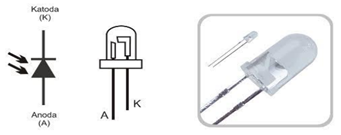
\includegraphics{Images/Fotodioda.png}
    \caption{Lambang dan Gambar Fotodioda LED Inframerah}
    \label{fig:led photodiode}
\end{figure}

Fotodioda adalah suatu jenis dioda yang resistansinya akan berubah-ubah apabila terkena sinar
cahaya. Resistansi dari fotodioda dipengaruhi oleh intensitas cahaya yang diterimanya, semakin
banyak cahaya yang diterima maka semakin kecil resistansi dari fotodioda dan begitupula sebaliknya
jika semakin sedikit intensitas cahaya yang diterima oleh sensor fotodioda maka semakin besar nilai
resistansinya\cite{Setyaningsih2017,DendyArta2020}.

\begin{figure}[H]
    \centering
    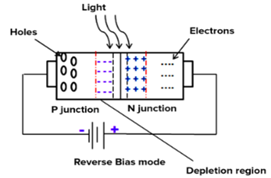
\includegraphics{Images/Bias Fotodioda.png}
    \caption{P-N Fotodioda}
    \label{fig:p-n photodiode}
\end{figure}

Pada fotodioda, terdapat bahan semikonduktor seperti \textit{silicon} (Si) atau \textit{gallium
arsenide} (GaAs) dan lain lain seperti \textit{indium antimonide} (InSb), \textit{lead selenide}
(PbSe) dan \textit{timah sulfida} (PbS). Fotodioda memiliki lapisan substrat dengan area depletion
sebagai tempat masuknya foton. Pada saat foton masuk ke area depletion, elektron pada N-substrat
akan bergerak membuat pasangan lubang-elektron pada katoda sehingga terjadi arus listrik pada
rangkaian fotodioda\cite{Vlasov2023}.

\begin{figure}[H]
    \centering
    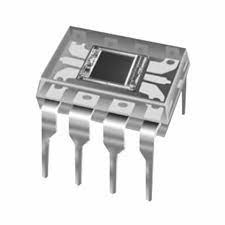
\includegraphics[width=5cm]{Images/OPT101.jpg}
    \caption{Fotodioda dengan \textit{Transimpedance Amplifier} OPT101}
    \label{fig:opt101}
\end{figure}

Pada prinsipnya fotodioda menghasilkan arus proporsional dari cahaya yang mengenai area aktif dari
fotodioda. Kebanyakan aplikasi dari pengukuran sensor ini menggunakan transimpedance amplifier
untuk mengkonversi nilai arus menjadi keluaran voltase. Adanya amplifier tersebut dapat
mengoperasikan fotodioda dalam mode \textit{photovoltaic} dimana op amp akan membuat voltase di
sekitar fotodioda pada 0V. Sebagai contoh terdapat pada OPT101 yang digunakan pada percobaan kali
ini.




\section{Mikrokontroler}
Mikrokontroler merupakan perangkat yang memiliki mikro prosesor dengan memori program dan memori
serbaguna, lalu didukung oleh fasilitas pendukung lainnya seperti output berupa data ke display
layaknya komputer dalam sebuah satu chip komputer sehingga mikrokontroler biasa disebut dengan
\textit{single chip computer}. Mikrokontroler ini dapat mengkontrol atau mengendalikan sebuah sistem
yang telah diprogram dalam chip tersebut. Berbeda dengan mikroprosesor dimana dalam mikrokontroler
ini terdapat komponen mikroprosesor yang didukung ADC, PPL, dan EEPROM dalam satu kemasan
\cite{Sokop2016}.

\begin{figure}[H]
    \centering
    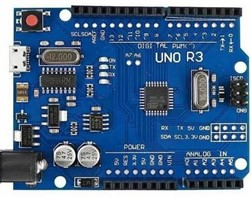
\includegraphics{Images/ArduinoUno.jpg}
    \caption{Board Arduino Uno R3}
    \label{fig:arduino}
\end{figure}

Dalam penelitian ini mikrokontroler yang digunakan merupakan mikrokontroler Arduino yang merupakan
platform komputasi fisik berbasiskan open source yang memiliki rangkaian input/output sederhana
dalam mengimplementasikan bahasa processing. Rangkaian ini memiliki IDE (\textit{Integrated 
Development Environment}) yang bersifat open source sehingga komponen dapat terhubung dengan
komponen lainnya tanpa bantuan alat lainnya. Pada perancangannya digunakan papan Arduino Uno R3
yang merupakan board mikrokontroler yang didasasrkan pada ATmega328\cite{Sokop2016}. Spesifikasi
dari Arduino Uno R3 sendiri yaitu:
\begin{longtable}{p{6cm}p{3pt}p{6cm}}
    \hspace{20pt} Mikrokontroller &:& ATmega328\\
    \hspace{20pt} Tegangan Pengoperasian &:&5 V\\
    \hspace{20pt} Tegangan Input Rekomendasi &:& 7-12V\\
    \hspace{20pt} Batas Tegangan Input &:& 6-20V\\
    \hspace{20pt} Jumlah Pin I/O Digital &:& 14\\
    \hspace{20pt} Jumlah Pin Input Analog &:& 6\\
    \hspace{20pt} Arus DC tiap Pin I/O &:& 40mA\\
    \hspace{20pt} Arus DC untuk Pin 3.3V &:& 50mA\\
    \hspace{20pt} Memori &:& 32 KB (ATmega328), sekitar 0.5KB digunakan oleh bootloader\\
    \hspace{20pt} SRAM &:& 2KB (ATmega328)\\
    \hspace{20pt} EEPROM &:& 1KB (ATmega328)\\
    \hspace{20pt} Clock Speed &:& 16 MHz
\end{longtable}

    \chapter{METODE PENELITIAN}
Bab ini akan menjelaskan mengenai tahapan penelitian dan pengujian komponen untuk perancangan
instrumen \textit{Dynamic Light Scattering} dan perencanaan pengolahan data yang dilakukan
dengan Arduino dan Python.


\section{Diagram Alir Penelitian}
Penelitian ini menggunakan metodologi yang dapat ditunjukan dengan diagram alir
berikut.

\begin{figure}[H]
    \centering
    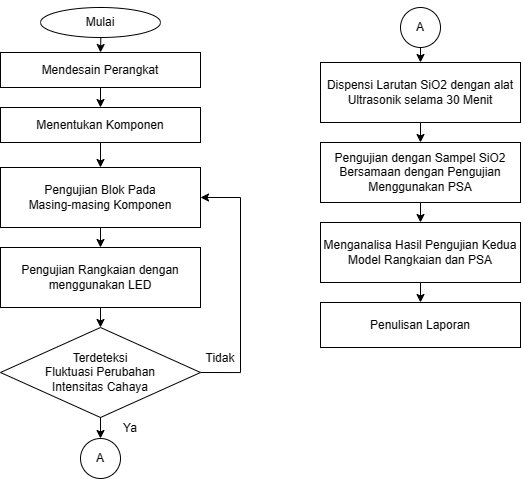
\includegraphics[width=12cm]{Images/Skema Penelitian.png}
    \caption{Diagram Alir Penelitian}
    \label{fig:reschart}
\end{figure}
\noindent Langkah-langkah pada gambar ~\ref{fig:reschart} dijelaskan sebagai berikut.

\begin{enumerate}
    \item Mendesain Perangkat agar dapat memastikan komponen yang dapat digunakan. Desain dari
    perangkat dibuat berdasarkan referensi yang didapatkan. Untuk membuat ruang gelap digunakan
    wadah hitam yang digunakan sebagai tempat pengukuran partikel dengan fotodioda. Untuk
    meminimalisir cahaya luar masuk ke sistem didalam ruang gelap, maka Arduino diposisikan
    di luar wadah.
    \item Menentukan Komponen. Berdasarkan desain yang telah dibuat, penentuan komponen dilakukan
    untuk menyesuaikan kebutuhan sesuai dengan spesifikasi yang dibutuhkan pada setiap proses
    pengambilan data. OPT101 digunakan sebagai fotodioda yang terintegrasi dengan
    \textit{Transimpedance Amplifier} sehingga tidak memerlukan Amplifier external sebagai filter
    aktif. Laser yang digunakan adalah modul laser merah 650nm dan modul laser hijau 532nm.
    \item Pengujian Blok pada Masing-masing komponen dilakukan untuk meminimalisir error yang
    dapat terjadi akibat dari salah satu komponen rangkaian. Setiap komponen diuji dengan
    menggunakan \textit{multimeter} dan \textit{power supply} untuk memastikan keluaran dari
    komponen.
    \item Rangkaian yang telah dirakit diuji dengan LED terlebih dahulu untuk memastikan
    apakah nilai keluaran sesuai dengan referensi. Nilai keluaran akan diproses dengan ADC
    \textit{(Analog Digital Converter)} dari sinyal pada sensor dan \textit{Transimpedance Amplifier}
    yang terdapat pada Arduino.
    \item Pengujian dengan sampel dilakukan bersamaan dengan pengujian pada PSA dari Horiba
    tipe SZ-100V2 pada ruangan
    dan suhu yang sama. Sampel yang digunakan merupakan ${SiO_2}$\cite{MadeJoni2020}
    berkarakteristik silika amorfus yang telah di ultrasonik selama 30 menit.
    \item Analisa Hasil Pengujian. Setelah didapatkan data dari kedua hasil pengujian, maka dilakukan
    analisa.
    \item Penulisan Laporan dilakukan sebagai bukti hasil yang didapat setelah melakukan penelitian.

\end{enumerate}


\section{Perancangan \textit{Prototype} Instrumen}

\subsection{Desain Sistem Instrumen DLS}

Rancangan dari rangkaian \textit{Dynamic Light Scattering} sederhana dengan dua laser yang
dibuat pada penelitian ini dapat digambarkan dengan Gambar ~\ref{fig:schemacirc}. Sistem dari
DLS dibuat dalam sebuah wadah tertutup gelap agar cahaya dari lingkungan tidak masuk kedalam
sistem. Laser merah dan Laser hijau diletakan menghadap kuvet, lalu diletakan stopper pada
salah satu sisi agar cahaya laser tidak terpantul kembali ke kuvet. Agar kedua laser dapat
digunakan bergantian, masing-masing laser dihubungkan dengan switch yang terhubung
dengan pin 5V dari arduino. Pada saat laser ditembakan ke kuvet, berkas cahaya laser yang
terhamburkan oleh partikel pada kuvet akan terdeteksi sensor fotodioda yang diletakan pada
sudut ${90\degree}$ dari sudut datang laser. Data yang diterima sensor lalu dikirim menuju Arduino
sebagai ADC dan diolah kembali pada program Python hingga didapatkan hasil pengukurannya.
\begin{figure}[H]
    \centering
    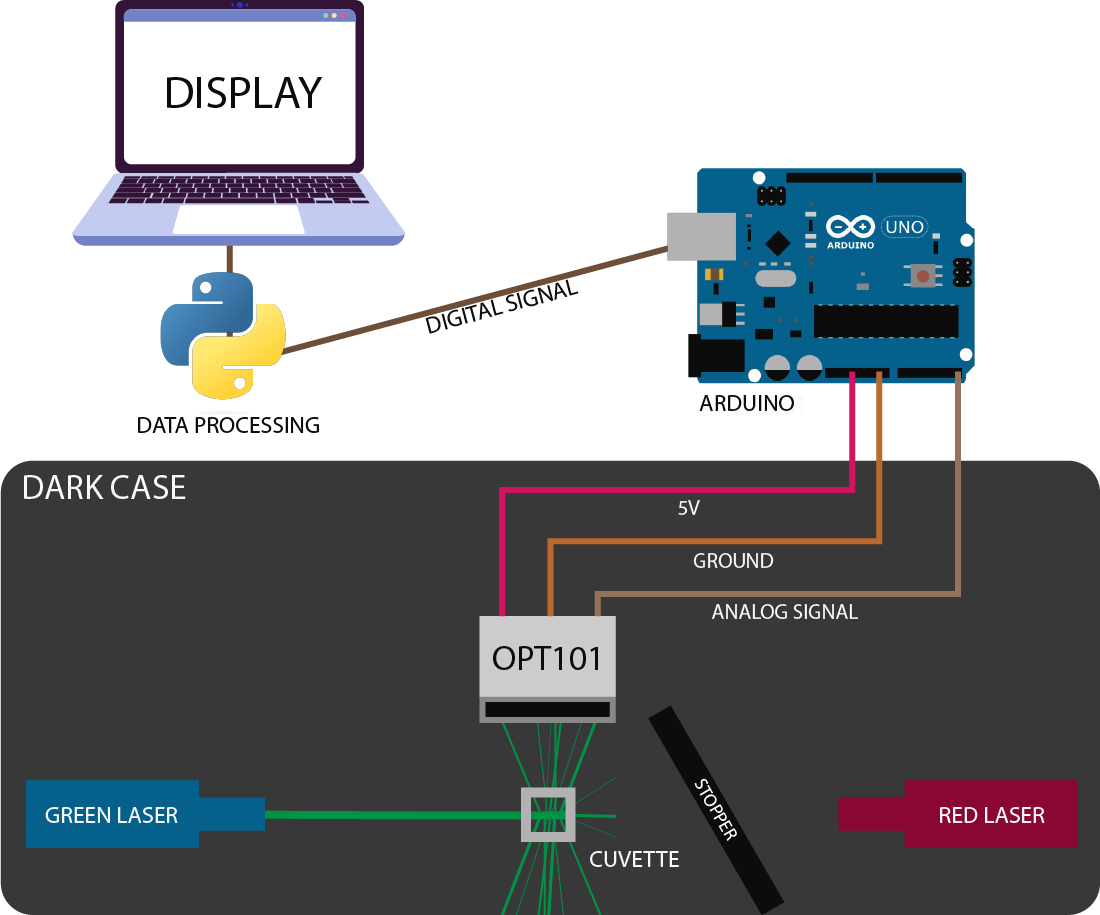
\includegraphics[width=14cm]{Images/Schema.png}
    \caption{Desain Rangkaian Instrumen DLS dua laser}
    \label{fig:schemacirc}
\end{figure}
\noindent
\textit{Transimpedance Amplifier} yang terdapat pada OPT101 dapat digambarkan dengan
diagram berikut yang bersumber dari datasheet \textit{Texas Instruments}
\begin{figure}[H]
    \centering
    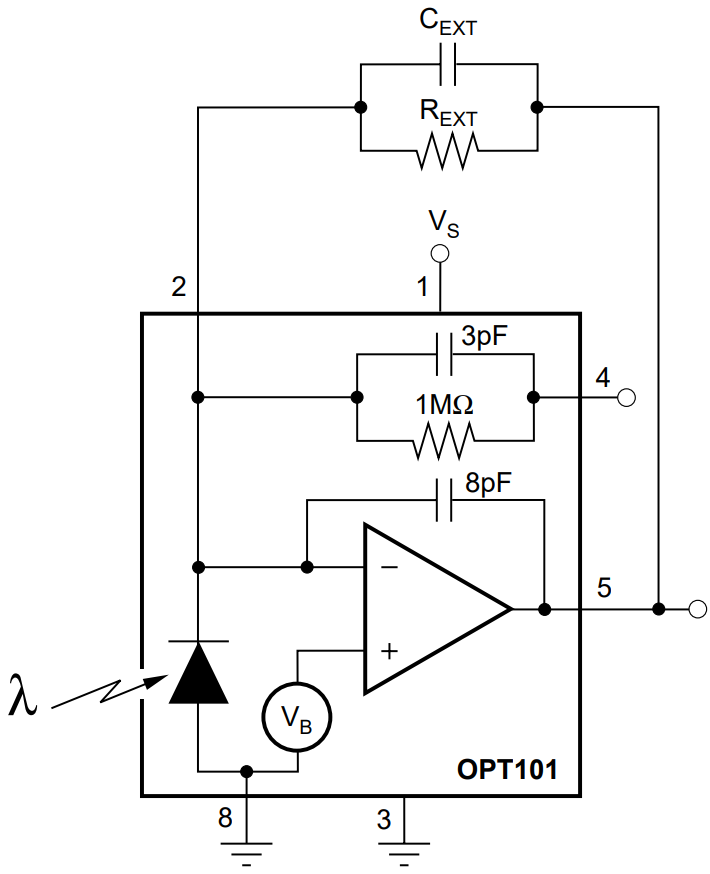
\includegraphics[width=8cm]{Images/Schema OPT101.png}
    \caption{Desain Rangkaian OPT101 (\textit{Texas Instruments})}
    \label{fig:schemaopt101}
\end{figure}
\noindent
Resistor Eksternal ${\left(R_{EXT} \right)}$ pada pengukuran partikel memiliki nilai
${10M \Omega}$ tanpa menggunakan Kapasitor Eksternal ${\left(C_{EXT}\right)}$. Namun untuk
memastikan pembesaran pada Amplifier sesuai, maka akan dilakukan
pengujian blok dengan variasi nilai Resistor Eksternal lainya.



\subsection{Diagram Blok Rangkaian}
\begin{figure}[H]
    \centering
    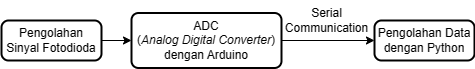
\includegraphics[width=12cm]{Images/Block Diagram.png}
    \caption{Diagram Blok Rangkaian DLS Sederhana}
    \label{fig:blockdiag}
\end{figure}

Diagram ~\ref{fig:blockdiag} dapat dijelaskan sebagai berikut.

\begin{enumerate}
    \item Pada instrumen DLS yang dibuat menggunakan fotodioda yang digunakan untuk mendeteksi
    hamburan cahaya dari pergerakan partikel. Fotodioda yang digunakan sudah terhubung dengan
    \textit{Transimpedance Amplifier} sehingga sinyal dari fotodioda dapat diperkuat untuk
    meningkatkan sensitivitas dari sensor tersebut.

    \item Sinyal yang keluar dari sistem fotodioda merupakan sinyal Analog sehingga untuk
    mengubahnya menjadi sinyal digital diperlukan ADC yang sudah terintegrasi pada Arduino.
    Sinyal dari Fotodioda terhubung dengan Arduino pada pin input A0.

    \item Sinyal yang telah diubah pada arduino disimpan, lalu dikirim menuju device seperti
    laptop. Device tersebut menerima data dengan serial communication
    dari Arduino. Data yang diterima akan diolah dengan program Python sehingga
    didapatkan nilai ukuran partikel.
\end{enumerate}


\subsection{Hasil Rancangan \textit{Prototype} Instrumen DLS}
Rangkaian DLS sederhana dua laser ini terdiri dari sebuah wadah \textit{casing} berbentuk balok
yang terbuat dari \textit{polymer} berwarna hitam dengan dimensi ${21.5 \times }$
${14.5 \times 8.5cm}$. Untuk mengurangi cahaya luar masuk ke sistem fotodioda digunakan sekat
yang membatasi kuvet dengan laser. Hasil rancangan alat tersebut dapat dilihat pada gambar
~\ref{fig:prot}.
\begin{figure}[H]
    \centering
    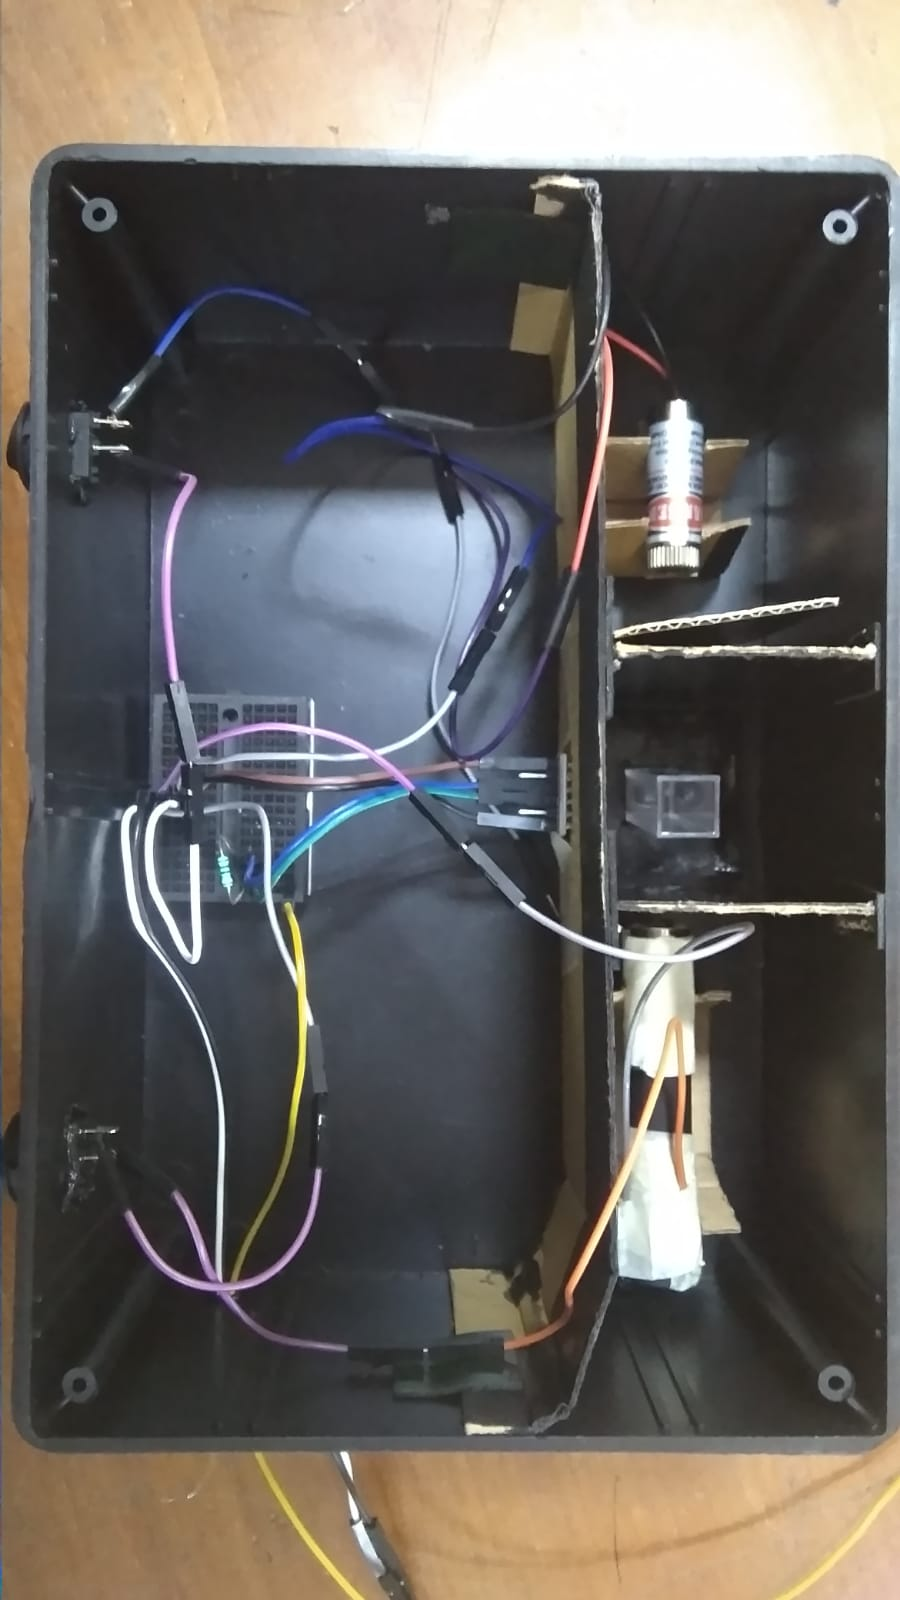
\includegraphics[width=12cm]{Images/Rangkaian.jpg}
    \caption{\textit{Prototype} Instrumen DLS Sederhana Dua Laser}
    \label{fig:prot}
\end{figure}

\noindent
Untuk menggunakan laser secara bergantian, setiap laser dihubungkan dengan switch
sehingga pada saat salah satu laser digunakan, laser lainnya dapat dimatikan untuk
mengurangi cahaya lingkungan masuk ke sistem.



\section{Desain Software}

\subsection{Pengolahan Data pada Arduino}
Penjelasan sistematika pengolahan data sensor pada arduino digambarkan pada gambar
~\ref{fig:schemaard}

\begin{figure}[H]
    \centering
    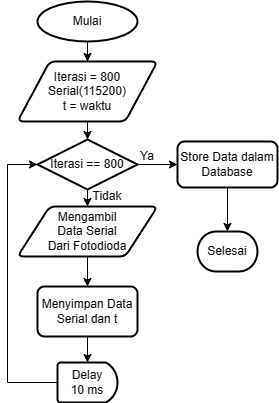
\includegraphics[width=8cm]{Images/Skema Arduino.png}
    \caption{Skema Pengolahan Data pada Arduino}
    \label{fig:schemaard}
\end{figure}
Sinyal yang keluar dari rangkaian fotodioda dan \textit{Transimpedance Amplifier} masuk melalui
pin input A0 Arduino. Sinyal tersebut diolah menjadi sinyal digital sehingga dapat dibaca dalam
bentuk angka pada komputer. Kecepatan pembacaan data dari sensor diatur dengan serial Arduino
yang pada penelitian ini optimumnya menggunakan \textit{baudrate} 115200. Spesifikasi dari
Arduino Uno R3 memiliki kapasitas penyimpanan dalam satu iterasi kurang lebih sebanyak 800
data dan akan dibangun dalam bentuk \textit{array}. Durasi iterasi penyimpanan data ditetapkan
sebagai variabel ${t}$.



\subsection{Pengolahan Data pada Python}
Ketika Arduino terhubung dengan laptop atau perangkat pengolahan data, setiap iterasi akan diolah
oleh program Python. Dengan menggunakan library \textit{Serial Communication}, pengiriman data
akan berjalan secara otomatis selama Arduino terhubung dengan laptop. Pengolahan data yang
diterima oleh laptop dapat digambarkan pada gambar ~\ref{fig:schemapy}

\begin{figure}[H]
    \centering
    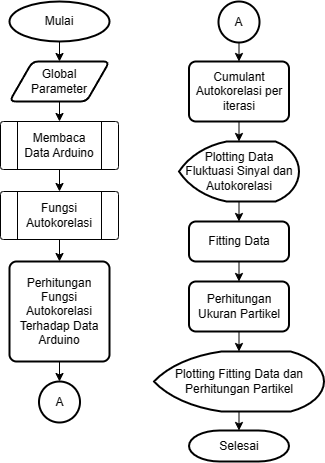
\includegraphics[width=9cm]{Images/Skema Python.png}
    \caption{Skema Pengolahan Data pada Python}
    \label{fig:schemapy}
\end{figure}

Data yang diterima program Python berupa 800 nilai dari pembacaan sensor dalam waktu ${t}$
didefinisikan sebagai \textit{Global Parameter}. Selain itu terdapat nilai Panjang gelombang
Laser, Indeks Bias, Konstanta Boltzman, Suhu sampel, Viskositas Sampel, dan Sudut Hamburan.
Nilai sensor yang dikirim melalui Serial akan diolah menggunakan Metode Kumulan Autokorelasi
dengan menggunakan \textit{numpy corelate}. Dalam persamaan matematis, Fungsi Autokorelasi
dapat dituliskan sebagai berikut:
\begin{equation}
    \hat{\gamma} = \frac{1}{n} \sum_{t=1}^{n-k}\left(y_t - \bar{y}\right)\left(y_{t+k} - \bar{y}\right)
\end{equation}
\noindent
dengan aturan fungsi ini dijalankan hingga nilai ${k}$ dimana ${k}$ sama dengan ${n-1}$

Data hasil autokorelasi tersebut tersimpan dalam bentuk
\textit{array}, lalu di plotting sehingga dapat dilakukan fitting data untuk mencari nilai
${c}$ yang mengacu pada persamaan~\ref{eq:c}. Kemudian perhitungan ukuran partikel
dilakukan dengan persamaan~\ref{eq:rh} untuk mencari nilai jari-jari partikel
berdasarkan nilai ${c}$.


\section{Pengambilan Data}
Pengujian alat dilakukan dengan menggunakan sampel \textit{Silika Geothermal} (${SiO_2}$)
\cite{MadeJoni2020} berkarakteristik silika amorfus yang dipanaskan dengan suhu rendah
(${70\degree C - 90\degree C}$) yang
telah di ultrasonik selama 30 menit agar distribusi ukuran partikel dalam pelarut homogen.
Pengambilan data dari DLS sederhana dilakukan bersamaan dengan karakterisasi menggunakan PSA
pada suhu ruangan (${20\degree C}$).

\subsection{Pengukuran dengan DLS Sederhana}
Data yang disimpan pada Arduino merupakan fluktuasi intensitas hamburan cahaya yang terdeteksi
pada sensor terhadap waktu. Data tersebut dijadikan variabel untuk perhitungan autokorelasi
hingga perhitungan ukuran partikel. Pengujian pada setiap laser dilakukan secara bergantian.
Untuk memastikan bahwa perhitungan pada program sesuai, data awal dari sensor disimpan dalam
penyimpanan lokal.

Pengambilan data ukuran partikel dilakukan sebanyak 10.000 kali untuk setiap laser. Total data
ukuran partikel berjumlah 20.000. Semua data yang terkumpul tercatat sebagai distribusi
ukuran partikel untuk masing-masing laser.

\subsection{Karakterisasi Sampel dengan PSA}
Pada waktu yang sama dilakukan karakterisasi psa untuk mengetahui distribusi ukuran partikel
sampel sebagai dasar untuk menganalisa kesesuaian data yang didapatkan dari DLS sederhana.
Data keluaran dari PSA berupa distribusi ukuran partikel dan \textit{Z-average} dari sampel
tersebut.
    \chapter{HASIL DAN PEMBAHASAN}

Dalam bab ini dibahas mengenai hasil perbandingan dari pengukuran
partikel berbasis Dynamic Light Scattering dengan menggunakan
PSA, DLS sederhana dengan laser merah dan hijau.

\section{Hasil Pengujian Blok OPT101}
Fotodioda yang digunakan dalam penelitian ini merupakan OPT101
yang di dalamnya sudah terkombinasi dengan \textit{transimpedance
amplifier} dalam satu chip nya sehingga mengurangi error yang
bersumber dari kebocoran arus. Oleh karena itu pengujian blok
hanya bisa dilakukan dengan memanfaatkan langsung fotodioda
sebagai input arus. Sebagai komparasi maka digunakan resistor
dengan nilai 1M${\Omega}$, 2M${\Omega}$, 3M${\Omega}$, 
4M${\Omega}$, 5M${\Omega}$, 10M${\Omega}$ dan untuk perubahan 
arus yang akan masuk digunakan LED yang input DC nya terhubung 
dengan power supply agar nilai Voltasenya dapat diatur untuk 
merubah intensitas cahaya dari LED. 

\begin{figure}[H]
  \centering
  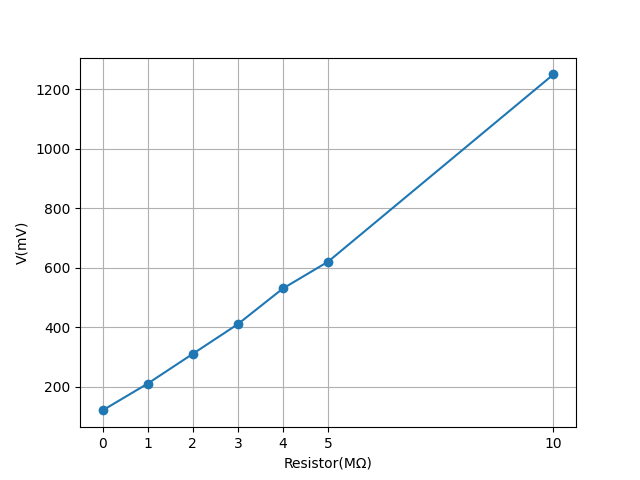
\includegraphics[width=12cm]{Images/Gain1.png}
  \caption{Nilai Output OPT101 terhadap Resistor}
  \label{fig:gain_res}
\end{figure}

Dari grafik diatas pembesaran nilai tegangan keluaran yang
dihasilkan dari rangkaian OPT101 menunjukan hasil yang linear
terhadap nilai resistor yang digunakan. IC yang tidak terhubung
dengan resistor memiliki nilai keluaran ${120mV}$, namun nilai
tersebut merupakan hasil yang ter invert sebelum melewati
rangkaian inverting sehingga perubahan nilai pada saat gelap
lebih tinggi dibandingkan saat lebih terang. Setelah diberikan
resistor secara inverting pada skema rangkaian \textit{Transimpedance
Amplifier}, nilai pembesaran yang diukur dengan menggunakan
persamaan:

\begin{equation}
  A_v = \frac{V_{output}}{V_{input}}
\end{equation}

didapatkan nilai 1,75 pada resistor 1M${\Omega}$, 2,58 pada
resistor 2M${\Omega}$, 3,41 pada resistor 3M${\Omega}$, 4,41
pada resistor 4M${\Omega}$, 5,16 pada resistor 5M${\Omega}$,
dan 10,41 pada resistor 10M${\Omega}$.

Untuk memastikan bahwa OPT101 mendeteksi perbedaan intensitas
cahaya maka dilakukan pengujian dengan memvariasikan intensitas
cahaya LED yang diletakan di depan fotodioda sehingga dihasilkan
data sebagai berikut

\begin{figure}[H]
  \centering
  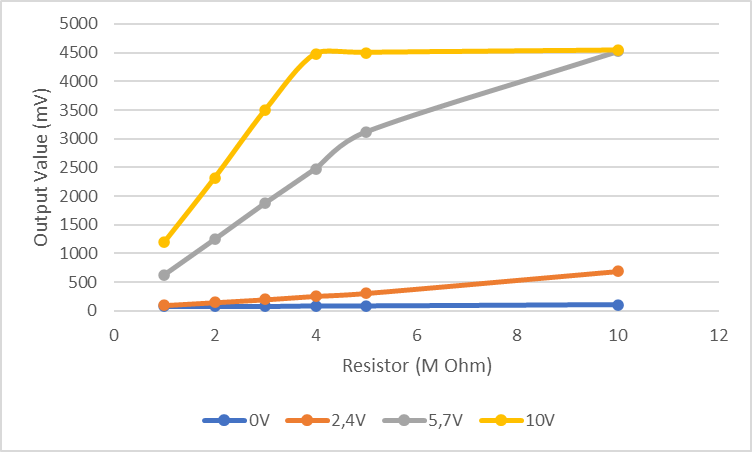
\includegraphics{Images/GainWLED.png}
  \caption{Nilai Output OPT101 terhadap Resistor}
  \vspace*{1.75pt}
  \caption*{dengan Variasi LED berbeda Intensitas Cahaya}
  \label{fig:gain_led}
\end{figure}

Pada saat LED tidak diberikan tegangan, keluaran dari OPT101 di
semua ukuran resistor hampir berdekatan pada kisaran ${70mV}$
hingga ${110mV}$. Ketika LED diberikan tegangan ${2,4V}$,
keluaran dari OPT101 pada setiap ukuran resistor memiliki
peningkatan sesuai gain oleh ukuran resistornya. LED yang
diberikan tegangan ${5,7V}$ dan ${10V}$ memiliki intensitas
cahaya yang lebih tinggi, namun data menunjukan adanya nilai
maksimum yang dibatasi oleh fotodiodanya. Output Value yang
dihasilkan dari OPT101 hanya dibatasi hingga nilai ${4500mV}$
sehingga pembesaran yang melebihi nilai ${4500mV}$ akan memiliki
nilai yang menyerupai nilai maksimum tersebut.


\section{Hasil Pengujian Instrumen Dynamic Light Scattering}
Kedua rangkaian alat yang digunakan merupakan modul rangkaian
dengan laser yang berbeda. Satu rangkaian menggunakan laser
merah dan rangkaian lainnya menggunakan laser hijau. Pada
pengujian ini digunakan sampel ${SiO_2}$ dengan pelarut aquades.

\subsection{Data Fluktuasi Sinyal}
Untuk memastikan kesesuaian data dari setiap pengukuran, maka
dilakukan beberapa pengukuran untuk membandingkan distribusi
persebaran ukuran partikel setiap waktunya dari masing-masing
laser.

\begin{figure}[H]
  \noindent
  \centering
  \begin{longtable}{p{7cm}p{7cm}}
    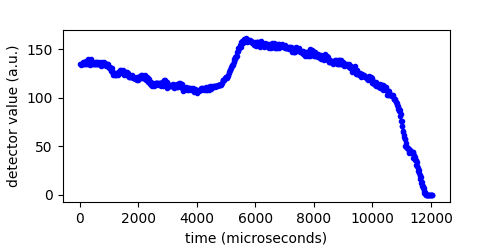
\includegraphics[width=8cm]{Images/RawData_Hijau_Data10-01.png}
    &
    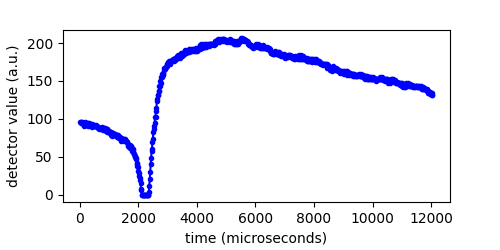
\includegraphics[width=8cm]{Images/RawData_Merah_Data9-01.png} \\
    
    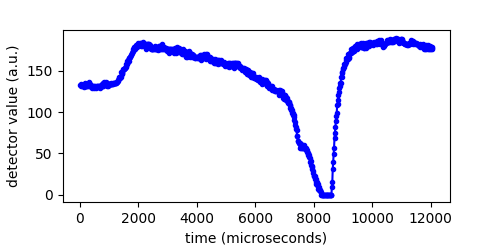
\includegraphics[width=8cm]{Images/RawData_Hijau_Data100-01.png}
    &
    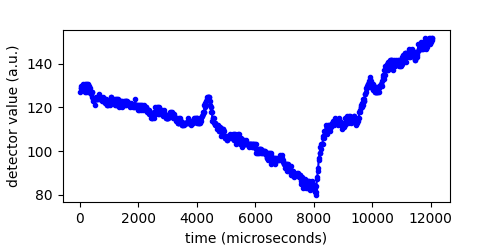
\includegraphics[width=8cm]{Images/RawData_Merah_Data99-01.png} \\
   
  \end{longtable}
\end{figure}
\begin{figure}
  \ContinuedFloat
  \begin{longtable}{p{7cm}p{7cm}}
    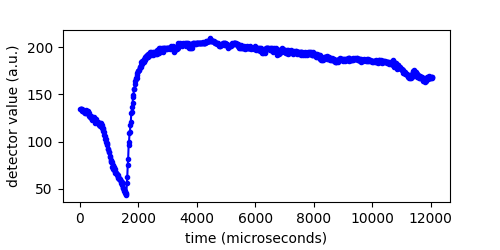
\includegraphics[width=8cm]{Images/RawData_Hijau_Data1000-01.png}
    \centering{Laser Hijau}
    &
    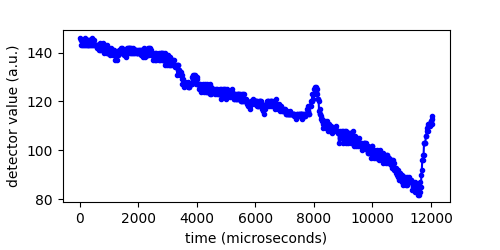
\includegraphics[width=8cm]{Images/RawData_Merah_Data1000-01.png} 
    \centering{Laser Merah}\\
  \end{longtable}

  \caption{Sampel Nilai Detektor Sensor terhadap Waktu}
\end{figure}

Grafik diatas menunjukkan beberapa data fluktuasi yang diukur
melalui 10.000 pengulangan dengan 800 nilai pada setiap
pengulangan dalam durasi 12.048 mikrodetik pada masing-masing
laser. Melalui grafik dapat dilihat bahwa fluktuasi yang
dihasilkan berbeda pada masing-masing laser, data yang terbaca
oleh sensor dari hamburan partikel menggunakan laser hijau
memiliki pola fluktuasi yang lebih bervariasi dibandingkan
dengan laser merah yang seringkali tidak mendeteksi perubahan
yang signifikan. Pada rangkaian laser merah  fluktuasi yang
dihasilkan memiliki pola yang hampir serupa pada setiap
pengukurannya.

Selain itu melalui grafik juga dapat diketahui bahwa hamburan
dari laser hijau memiliki fluktuasi yang cukup cepat, dapat
diperlihatkan dari seberapa cepat detektor mencapai lembah dan
kembali lagi ke puncak, sedangkan hamburan dari laser merah
dominan memiliki perubahan yang lebih lambat.

\subsection{Data Autokorelasi}
Fluktuasi nilai dari sensor pada setiap pengukurannya dapat
dijadikan acuan sebagai seberapa cepat partikel tersebut
bergerak. Untuk mendapatkan nilai ukuran partikel diperlukan
nilai autokorelasi yang merupakan korelasi dari setiap nilai
pada setiap pengulangan. Nilai autokorelasi didapatkan dengan
menggunakan \textit{library Numpy} dari Python untuk mempermudah
pengolahan data berbentuk matriks. Dari nilai autokorelasi
terebut dapat di plotting menjadi gambar berikut:

\begin{figure}[H]
  \noindent
  \centering
  \begin{longtable}{p{7cm}p{7cm}}
    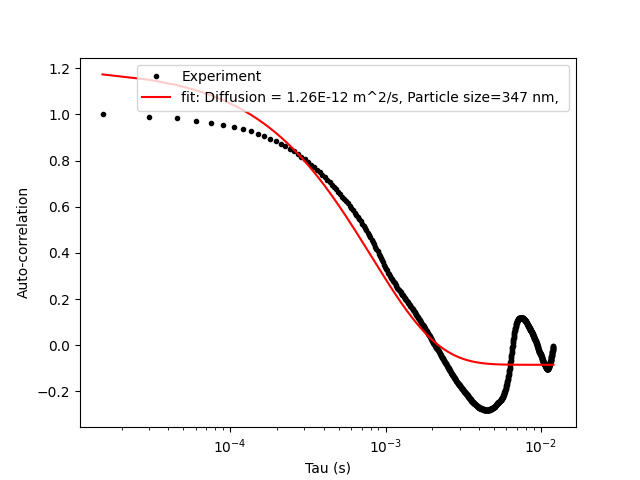
\includegraphics[width=8cm]{Images/AutoCor_Hijau_Data10-01.png}
    &
    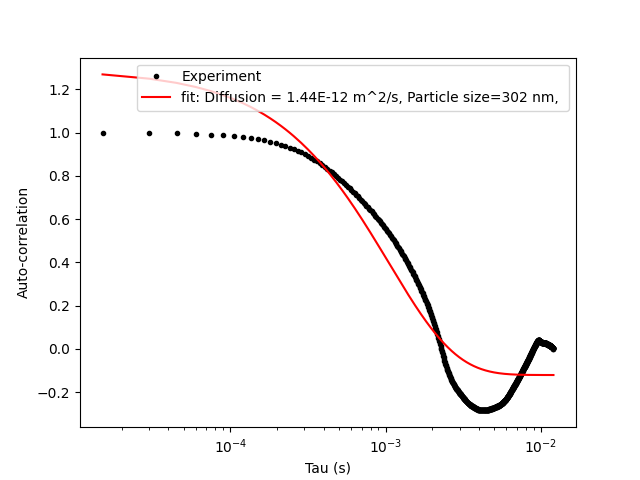
\includegraphics[width=8cm]{Images/AutoCor_Merah_Data9-01.png} \\
    
    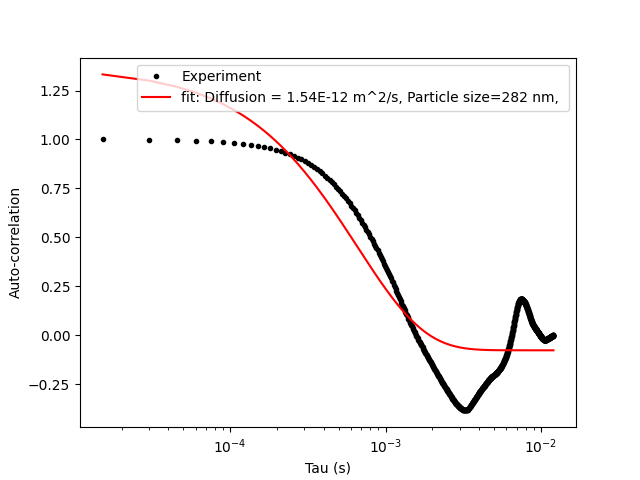
\includegraphics[width=8cm]{Images/AutoCor_Hijau_Data100-01.png}
    &
    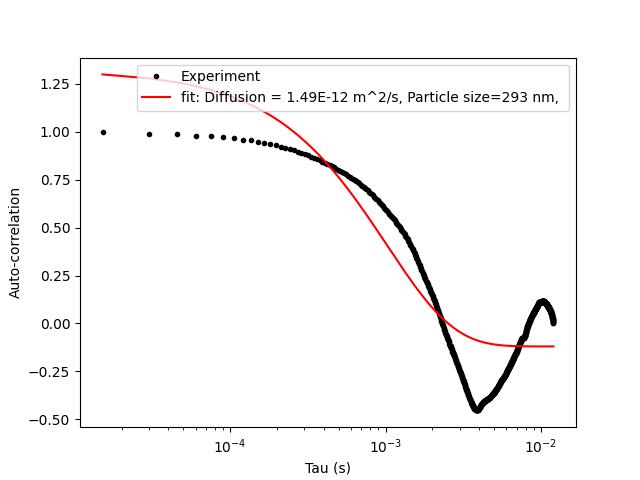
\includegraphics[width=8cm]{Images/AutoCor_Merah_Data99-01.png} \\
   
  \end{longtable}
\end{figure}
\begin{figure}
  \ContinuedFloat
  \begin{longtable}{p{7cm}p{7cm}}
    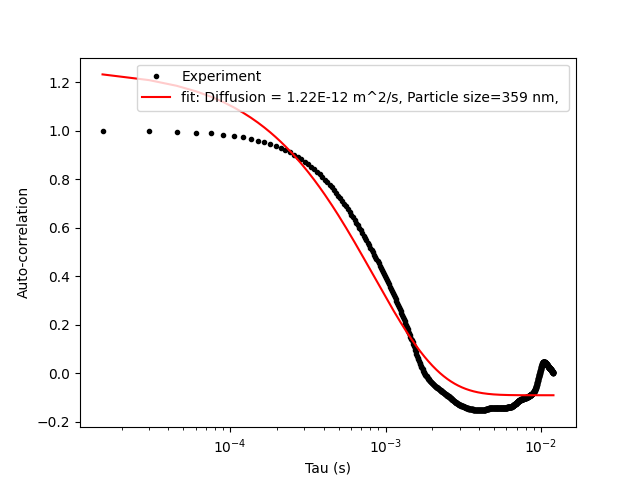
\includegraphics[width=8cm]{Images/AutoCor_Hijau_Data1000-01.png}
    \centering{Laser Hijau}
    &
    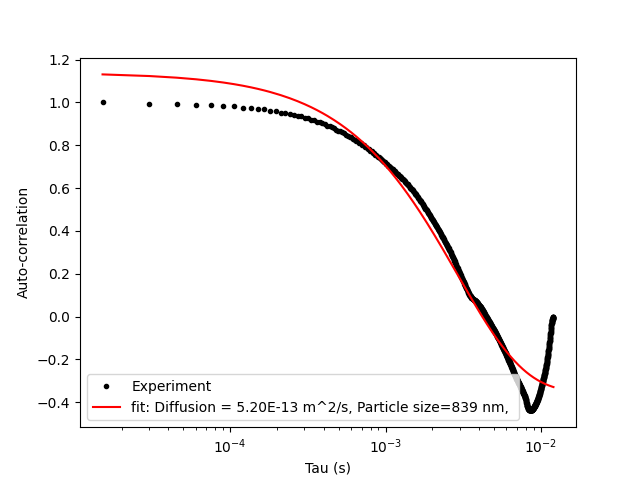
\includegraphics[width=8cm]{Images/AutoCor_Merah_Data1000-01.png} 
    \centering{Laser Merah}\\
  \end{longtable}

  \caption{Sampel Data Autokorelasi terhadap Tau}
\end{figure}


\subsection{Hasil Karakterisasi Sampel pada PSA}
\begin{figure}[H]
  \centering
  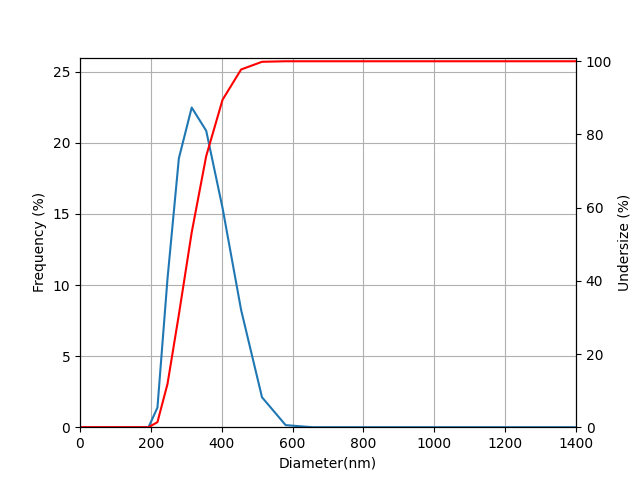
\includegraphics[width=10cm]{Images/DistribusiPSA.png}
  \caption{Distribusi Ukuran Partikel pada PSA}
  \label{fig:psa}
\end{figure}
Pada pengukuran PSA, data yang didapat berupa ${Z-Average}$ berkisar
di ${251 nm}$ dengan PI 2,555. Data tersebut mempengaruhi pengukuran
dari PSA karena Polidyspersity Index yang tinggi mengurangi tingkat
akurasi pada pengukuran. Apabila dibandingkan dengan kedua rangkaian
DLS yang diuji, distribusi data diameter partikel yang didapat
memiliki range lebih sempit. Lebar range tersebut juga mempengaruhi
tingkat akurasi dari pengukuran pada rangkaian yang digunakan.


\subsection{Distribusi Data Ukuran Partikel}
\begin{figure}[H]
  \centering
  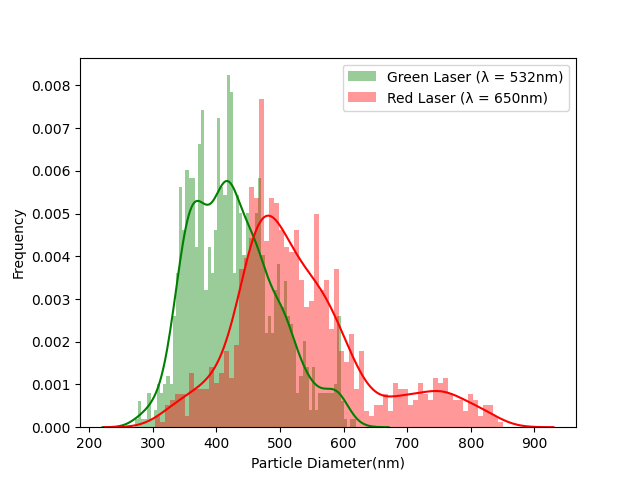
\includegraphics[width=13cm]{Images/Distribusi 10000x.png}
  \caption{Distribusi 20000 Ukuran Partikel}
  \label{fig:dist10000x}
\end{figure}

Grafik diatas merupakan grafik distribusi frekuensi terhadap
diameter dari partikel. Distribusi kedua data dengan 10.000
iterasi pada masing-masing laser memiliki perbedaan hasil
kumulatif yang cukup signifikan. Persebaran diameter partikel
dengan laser merah memiliki range yang lebar dengan beberapa
puncak, seperti yang terlihat pada grafik dimana diameter
partikel memiliki puncak pada rentang ${300nm-350nm}$ dan
${580nm-620nm}$. Adanya tiga puncak dari grafik distribusi diatas
menunjukan adanya tiga ukuran partikel yang terdeteksi. Perubahan
nilai pada sensor yang lambat menghasilkan perhitungan dimeter
partikel yang lebih besar, namun terdapat beberapa pengulangan
yang mendeteksi perubahan dengan cepat sehingga dapat mengukur
diameter partikel yang lebih kecil. Berbeda dengan laser hijau
yang memiliki persebaran diameter partikel yang memiliki puncak
pada rentang ${200nm-400nm}$. Range data yang terukur pada laser
hijau dominan lebih kecil dibandingkan pada laser merah. Hal ini
menunjukan bahwa laser hijau dapat mendeteksi diameter partikel
yang lebih kecil dibandingkan denga laser merah.

\begin{figure}[H]
  \centering
  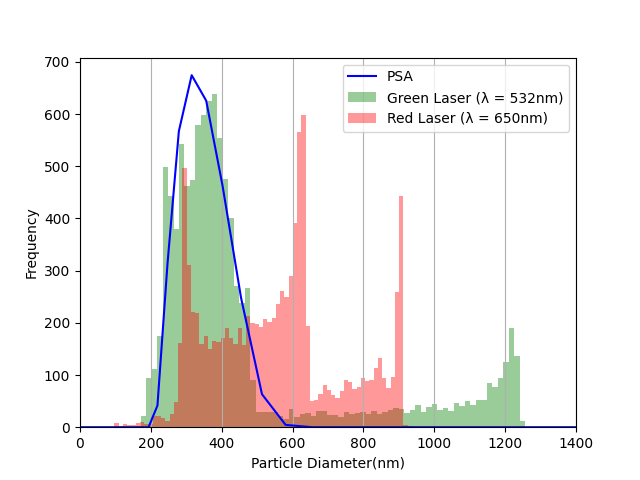
\includegraphics[width=13cm]{Images/DistribusiWithPSAHist.png}
  \caption{Perbandingan Hasil Instrumen dengan Karakterisasi PSA}
  \label{fig:distwpsa}
\end{figure}




% \section{Gambar}

% \begin{figure}[H]
%   \centering
%   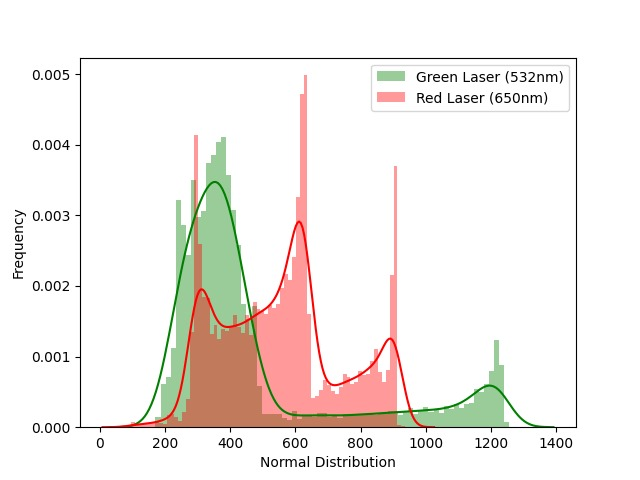
\includegraphics[width=8cm]{Images/Distribusi 1000x.jpg}
%   \caption{Contoh Gambar}
%   \label{fig:blg}
% \end{figure}

% \begin{enumerate}
%   \item Gambar dimuat kira-kira di tengah-tengah halaman.
%   \item Judulnya ditik di bawah gambar, mengikuti lebar gambar dengan memperhitungkan keseimbangan halaman.
%   \item Nomor gambar terdiri atas dua bagian, yaitu:
%   \begin{enumerate}[label=(\alph*)]
%     \item bagian pertama menunjukkan nomor bab tempat gambar itu dimuat;
%     \item bagian kedua menunjukkan nomor urut gambar pada bab itu. Misalnya, Gambar  \ref{fig:blg} menunjukkan bahwa gambar itu ada pada Bab IV dan merupakan gambar urutan pertama pada bab itu.
%   \end{enumerate}
%   \item Kalimat pertama judul gambar ditulis dengan jarak dua ketukan sesudah nomor gambar.
%   \item Awal baris kedua judul gambar berada di bawah awal judul gambar (bukan di bawah nomor gambar).
% \end{enumerate}

% \section{Grafik}
% \begin{figure}[H]
%   \begin{subfigure}{.5\textwidth}
%     \centering
%     \includegraphics[width=6.7cm]{Gambar/cv.pdf}
%   \end{subfigure}
%   \hspace{0.7em}
%   \begin{subfigure}{.5\textwidth}
%     \centering
%     \includegraphics[width=6.7cm]{Gambar/cv_comp.pdf}
%   \end{subfigure}
%   \caption{Contoh Grafik}
%   \label{fig:cv}
%   \end{figure}

% \begin{enumerate}
%   \item Grafik dimuat kira-kira di tengah-tengah halaman.
%   \item Judulnya ditik di atas grafik, mengikuti lebar grafik, dengan memperhitungkan keseimbangan halaman.
%   \item Nomor grafik terdiri atas dua bagian, yaitu:
%   \begin{enumerate}[label=(\alph*)]
%     \item bagian pertama menunjukkan nomor bab grafik itu dimuat; 
%     \item bagian kedua menunjukkan nomor urut grafik pada bab itu. Misalnya, Gambar  ~\ref{fig:cv} menunjukkan bahwa grafik itu ada pada Bab IV dan merupakan grafik urutan keempat pada bab itu.
%   \end{enumerate}
%   \item Kalimat pertama judul grafik ditulis dengan jarak dua ketukan sesudah nomor grafik.
%   \item Awal baris kedua judul grafik berada di bawah awal judul grafik (bukan di bawah nomor grafik).
% \end{enumerate}

% \section{Tabel}
% \begin{table}[ht!]
%   \centering
%   \caption{Contoh Tabel}
%   \begin{tabular}{|l|l|l|l|l|l|}
%   \hline
%   \textbf{Sistem} & \textbf{m, n} & \textbf{\begin{tabular}[c]{@{}l@{}}Sudut\\ Puntir (\degree)\end{tabular}} & \textbf{\begin{tabular}[c]{@{}l@{}}Duplikasi\\ ($x \times y \times z$)\end{tabular}} & \textbf{\begin{tabular}[c]{@{}l@{}}Panjang\\ Sistem (\AA)\end{tabular}} & \textbf{\begin{tabular}[c]{@{}l@{}}Jumlah\\ Atom\end{tabular}} \\ \hline
%   SLG             & -             & -                                                                  & 1 x 1 x 1                                                                & 35,98                                                                 & 434                                                            \\ \hline
%   BLG          & -             & 0                                                                  & 1 x 1 x 1                                                                & 35,98                                                                 & 868                                                            \\ \hline
%   tBLG            & 9, 8          & 3,89                                                               & 1 x 1 x 1                                                                & 35,98                                                                 & 868                                                            \\ \hline
%   tBLG            & 8, 7          & 4,41                                                               & 1 x 1 x 1                                                                & 31,75                                                                 & 676                                                            \\ \hline
%   tBLG            & 5, 3          & 16,43                                                              & 2 x 2 x 1                                                                & 34,20                                                                  & 784                                                            \\ \hline
%   \end{tabular}
%   \label{tab:str}
%   \end{table}

% \begin{enumerate}
%   \item Tabel dimuat kira–kira di tengah–tengah halaman.
%   \item Judulnya ditik di atas tabel, mengikuti lebar tabel, dengan memperhitungkan keseimbangan halaman.
%   \item Nomor tabel terdiri atas dua bagian, yaitu:
%   \begin{enumerate}[label=(\alph*)]
%     \item bagian pertama menunjukkan nomor bab tabel itu dimuat;
%     \item bagian kedua menunjukkan nomor urut tabel pada bab itu. Misalnya, Tabel ~\ref{tab:str} menunjukkan bahwa tabel itu berada pada Bab IV dan merupakan tabel urutan pertama pada bab itu.
%   \end{enumerate}
%   \item Kalimat pertama judul tabel ditulis dengan jarak dua ketukan sesudah nomor tabel.
%   \item Awal baris kedua judul tabel berada di bawah awal judul tabel (bukan di bawah nomor tabel).
%   \item Ukuran huruf pada isi tabel adalah 10 pt.
%   \item Isi tabel ditulis dalam 1 spasi.
% \end{enumerate}

% \section{Persamaan}

% \begin{equation}
%   U_{i j}^{\mathrm{LJ}}\left(r_{i j}\right)=4 \epsilon_{i j}\left[\left(\frac{\sigma_{i j}}{r_{i j}}\right)^{12}-\left(\frac{\sigma_{i j}}{r_{i j}}\right)^{6}\right]
% \end{equation}

% \begin{equation}
%   f_{Q}=\frac{C_v(T)}{3Nk_B}=\frac{\displaystyle\int\limits_{0}^{\infty}\frac{u^2e^u}{{(e^u-1)}^2}G(\omega)d\omega}{\displaystyle\int\limits_{0}^{\infty}G(\omega)d\omega}
% \end{equation}

% \section{Sitasi}
% Sitasi dapat dimasukkan seperti ini \cite{moore1998cramming}. Untuk sitasi dengan beberapa sumber, dapat dituliskan juga \cite{wang2020frank,zhang2020molecular}. Atau untuk tiga sumber seperti ini \cite{mcgaughey2019phonon,jiang2015graphene,khan2015equilibrium}.
    \chapter{KESIMPULAN DAN SARAN}

\section{Kesimpulan}
Telah dibandingkan dua instrument \textit{Dynamic Light Scattering} (DLS) sederhana dengan
laser yang berbeda yaitu laser merah dan laser hijau yang memiliki hasil berkisar diantara
${365 nm}$ untuk laser hijau dan ${398 nm}$ dan ${619 nm}$ untuk laser merah.
Sebagai referensi didapatkan data pengukuran PSA berupa Z-Average pada ${463.1 nm}$
\begin{enumerate}
    \item Laser merah memiliki range persebaran data yang lebih lebar dibandingkan
    dengan laser hijau. Disisi lain pengukuran dengan laser hijau menghasilkan diameter yang
    dominan lebih kecil dibandingkan laser merah.
    \item Responsivitas dari silikon pada fotodioda OPT101 memiliki nilai lebih rendah
    pada laser hijau dibandingkan dengan laser merah, namun intensitas dari laser hijau lebih
    sehingga sensitivitas pada sensor meningkat dibandingkan dengan laser merah
\end{enumerate}


\section{Saran}
Berdasarkan penelitian yang telah dilakukan, sampel yang dapat diukur masih terlalu
sedikit untuk memastikan akurasi pengukuran yang dilakukan oleh rangkaian yang telah
dibuat. Hal tersebut memberikan saran berupa adanya variasi sampel yang lebih banyak
namun masih dalam range pengukuran dengan menggunakan laser merah dan laser hijau
agar mendapatkan data yang beragam.

    \bibliographystyle{ieeetr}
    \bibliography{ref}
    \addcontentsline{toc}{chapter}{DAFTAR PUSTAKA}

    % \input{Isi/Lampiran}
\end{document}
